\subsection{平行公理}\label{subsec:czjh1-2-5}

我们先学习平行线的画法。

已知直线 $AB$ 和 $AB$ 外的一点 $P$, 经过点 $P$ 画平行于直线 $AB$ 的直线(图 \ref{fig:czjh1-2-15})。

\begin{figure}[htbp]
    \centering
    \begin{minipage}[b]{7cm}
        \centering
        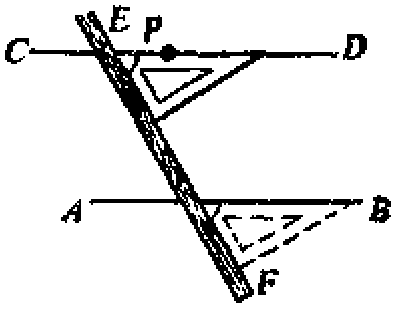
\includegraphics[width=5cm]{../pic/czjh1-ch2-15.png}
        \caption{}\label{fig:czjh1-2-15}
    \end{minipage}
    \qquad
    \begin{minipage}[b]{7cm}
        \centering
        \begin{tikzpicture}
    \tkzDefPoints{0/0/E, 2/0/F, 0/0.8/C, 2/0.8/D,  0/1.6/A,  2/1.6/B}
    \tkzInterCC(B,D)(D,B)   \tkzGetFirstPoint{P}

    \tkzDrawSegments(A,B  C,D  E,F)
    \tkzDrawArc[rotate, dashed](B,D)(80)
    \tkzDrawArc[rotate, dashed](D,B)(-80)
    \tkzDrawPoint(P)
    \tkzLabelPoints[left](A, C, E)
    \tkzLabelPoints[above](B)
    \tkzLabelPoints[below](D)
    \tkzLabelPoints[right](F, P)
\end{tikzpicture}


        \caption{}\label{fig:czjh1-2-16}
    \end{minipage}
\end{figure}

\huafa 1. 把三角板的一边靠紧 $AB$,再用直尺(或另一块三角板)靠紧三角板的另一边。

2. 沿直尺推动三角板,使原来和 $AB$ 重合的一边经过点 $P$。

3. 沿三角板的这条边画直线 $CD$。

$CD$ 就是所求的直线。

这样的直线可以画出一条,而且只能画出一条。

我们把这个事实作为公理:

\begin{gongli}[平行公理]
    经过直线外一点,有一条而且只有一直线和这条直线平行。
\end{gongli}

从平行公理可以推出:

\begin{xingzhi}
    如果两条直线都和第三条直线平行,那么这两条直线也互相平行。
\end{xingzhi}

例如,如果直线 $AB$ 与 $CD$ 都和直线 $EF$ 平行(图 \ref{fig:czjh1-2-16}),
那么 $AB$ 与 $CD$ 必定平行。这是因为,假如 $AB$ 与 $CD$ 不平行,
相交于点 $P$,那么过点 $P$ 就会有两条直线 $AB$ 与 $CD$ 都和 $EF$ 平行。
这是不符合平行公理的。


\begin{lianxi}

\xiaoti{照图的样子,先作线段 $OX = 50\;\haomi$, $OY = 50\;\haomi$, 并且使 $OX \perp OY$。
    再过 $X$、$Y$ 分别作 $OY$、$OX$ 的平行线,两线相交于 $A$。然后用刻度尺把 $OX$、$OY$ 各分成 10 等分,
    从 $OY$ 上每个分点作平行于 $OX$ 的线段,
    从 $OX$ 上每个分点作平行于 $OY$ 的线段。
}

\begin{figure}[htbp]
    \centering
    \begin{tikzpicture}
    \foreach \x in {0, .5, 1, ..., 5} {
        \tkzDefPoints{\x/0/A, \x/5/B}
        \tkzDrawSegment(A,B)
    }
    \foreach \y in {0, .5, 1, ..., 5} {
        \tkzDefPoints{0/\y/C, 5/\y/D}
        \tkzDrawSegment(C,D)
    }

    \tkzDefPoints{0/0/O, 5/0/X, 0/5/Y, 5/5/A}
    \tkzLabelPoints[left](O,Y)
    \tkzLabelPoints[right](X,A)
\end{tikzpicture}


    \caption*{(第 1 题)}
\end{figure}


\xiaoti{填空:$\because$ \quad $AB \pingxing EF$,$CD \pingxing EF$(已知),\\
    $\therefore$ \quad $\ewkh[4em] \pingxing \ewkh[4em] \quad \ewkh[8em]$。
}

\xiaoti{读下列语句,并画出图形:}
\begin{xiaoxiaotis}

    \xxt{点 $P$ 是直线 $AB$ 外的一点,直线 $CD$ 经过点 $P$,且与直线 $AB$ 平行;}

    \xxt{直线 $AB$、$CD$ 是相交直线, 点 $P$ 是直线 $AB$、$CD$ 外的一点,
        直线 $EF$ 经过点 $P$ 与直线 $AB$ 平行,与直线 $CD$ 相交于 $E$。
    }

\end{xiaoxiaotis}

\end{lianxi}
